\section{A Reta de Regressão e a Função de Perda}

\begin{frame}{Como Predizer $Y$ a Partir de $X$?}
    \begin{columns}
        \begin{column}{0.5\textwidth}
            \textbf{Abordagem Local (Média Condicional):}
            \begin{itemize}
                \item Agrupamos os dados em janelas verticais estreitas no eixo $X$.
                \item Calculamos a média amostral da variável $Y$ para cada janela.
                \item Funciona bem se houver abundância de dados em todos os intervalos de $X$.
            \end{itemize}
        \end{column}
        \begin{column}{0.5\textwidth}
            \textbf{Abordagem Global (Modelo Linear):}
            \begin{itemize}
                \item E se as janelas tiverem poucos dados (esparsa amostragem)?
                \item Buscamos uma reta global contínua que descreva a tendência geral.
                \item Esta linha reta é a chamada \textbf{Reta de Regressão}.
            \end{itemize}
        \end{column}
    \end{columns}
\end{frame}

\begin{frame}{Reta em Unidades Padrão (Z-Scores)}
    \begin{itemize}
        \item Definimos Z-score (unidades padrão) de uma variável como:
        $$x_{su} = \frac{x_i - \bar{X}}{s_x}, \quad y_{su} = \frac{y_i - \bar{Y}}{s_y}$$
        \item Onde $\bar{X}, \bar{Y}$ são as \textbf{Médias Amostrais} e $s_x, s_y$ são os \textbf{Desvios Padrão Amostrais}.
        \item Em unidades padrão, a reta de regressão assume uma forma extremamente elegante:
        $$\hat{y}_{su} = r \cdot x_{su}$$
        \item Características:
        \begin{itemize}
            \item Sempre cruza a origem das coordenadas $(0, 0)$.
            \item A inclinação (slope) da reta é exatamente o \textbf{Coeficiente de Correlação de Pearson} ($r$).
        \end{itemize}
    \end{itemize}
\end{frame}

\begin{frame}{Considere o Gráfico ao Lado}
    \begin{columns}
        \begin{column}{0.5\textwidth}
            \textbf{Sintético}
            \begin{itemize}
                \item A linha vermelha é a linha de 45 graus.
                \item \textbf{Qual é o valor do Coeficiente Angular ($\beta$)?}
            \end{itemize}
            \vspace{0.4cm}
            \centering
            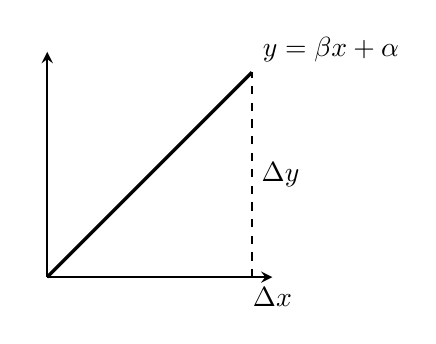
\begin{tikzpicture}[scale=1.3]
                \draw[->,>=stealth,thick] (0,0) -- (2.2,0) node[below] {$\Delta x$};
                \draw[->,>=stealth,thick] (0,0) -- (0,2.2) node[left] {};
                \draw[very thick] (0,0) -- (2,2) node[above right] {$y = \beta x + \alpha$};
                \draw[dashed] (2,0) -- (2,2) node[midway,right] {$\Delta y$};
            \end{tikzpicture}
        \end{column}
        \begin{column}{0.5\textwidth}
            \centering
            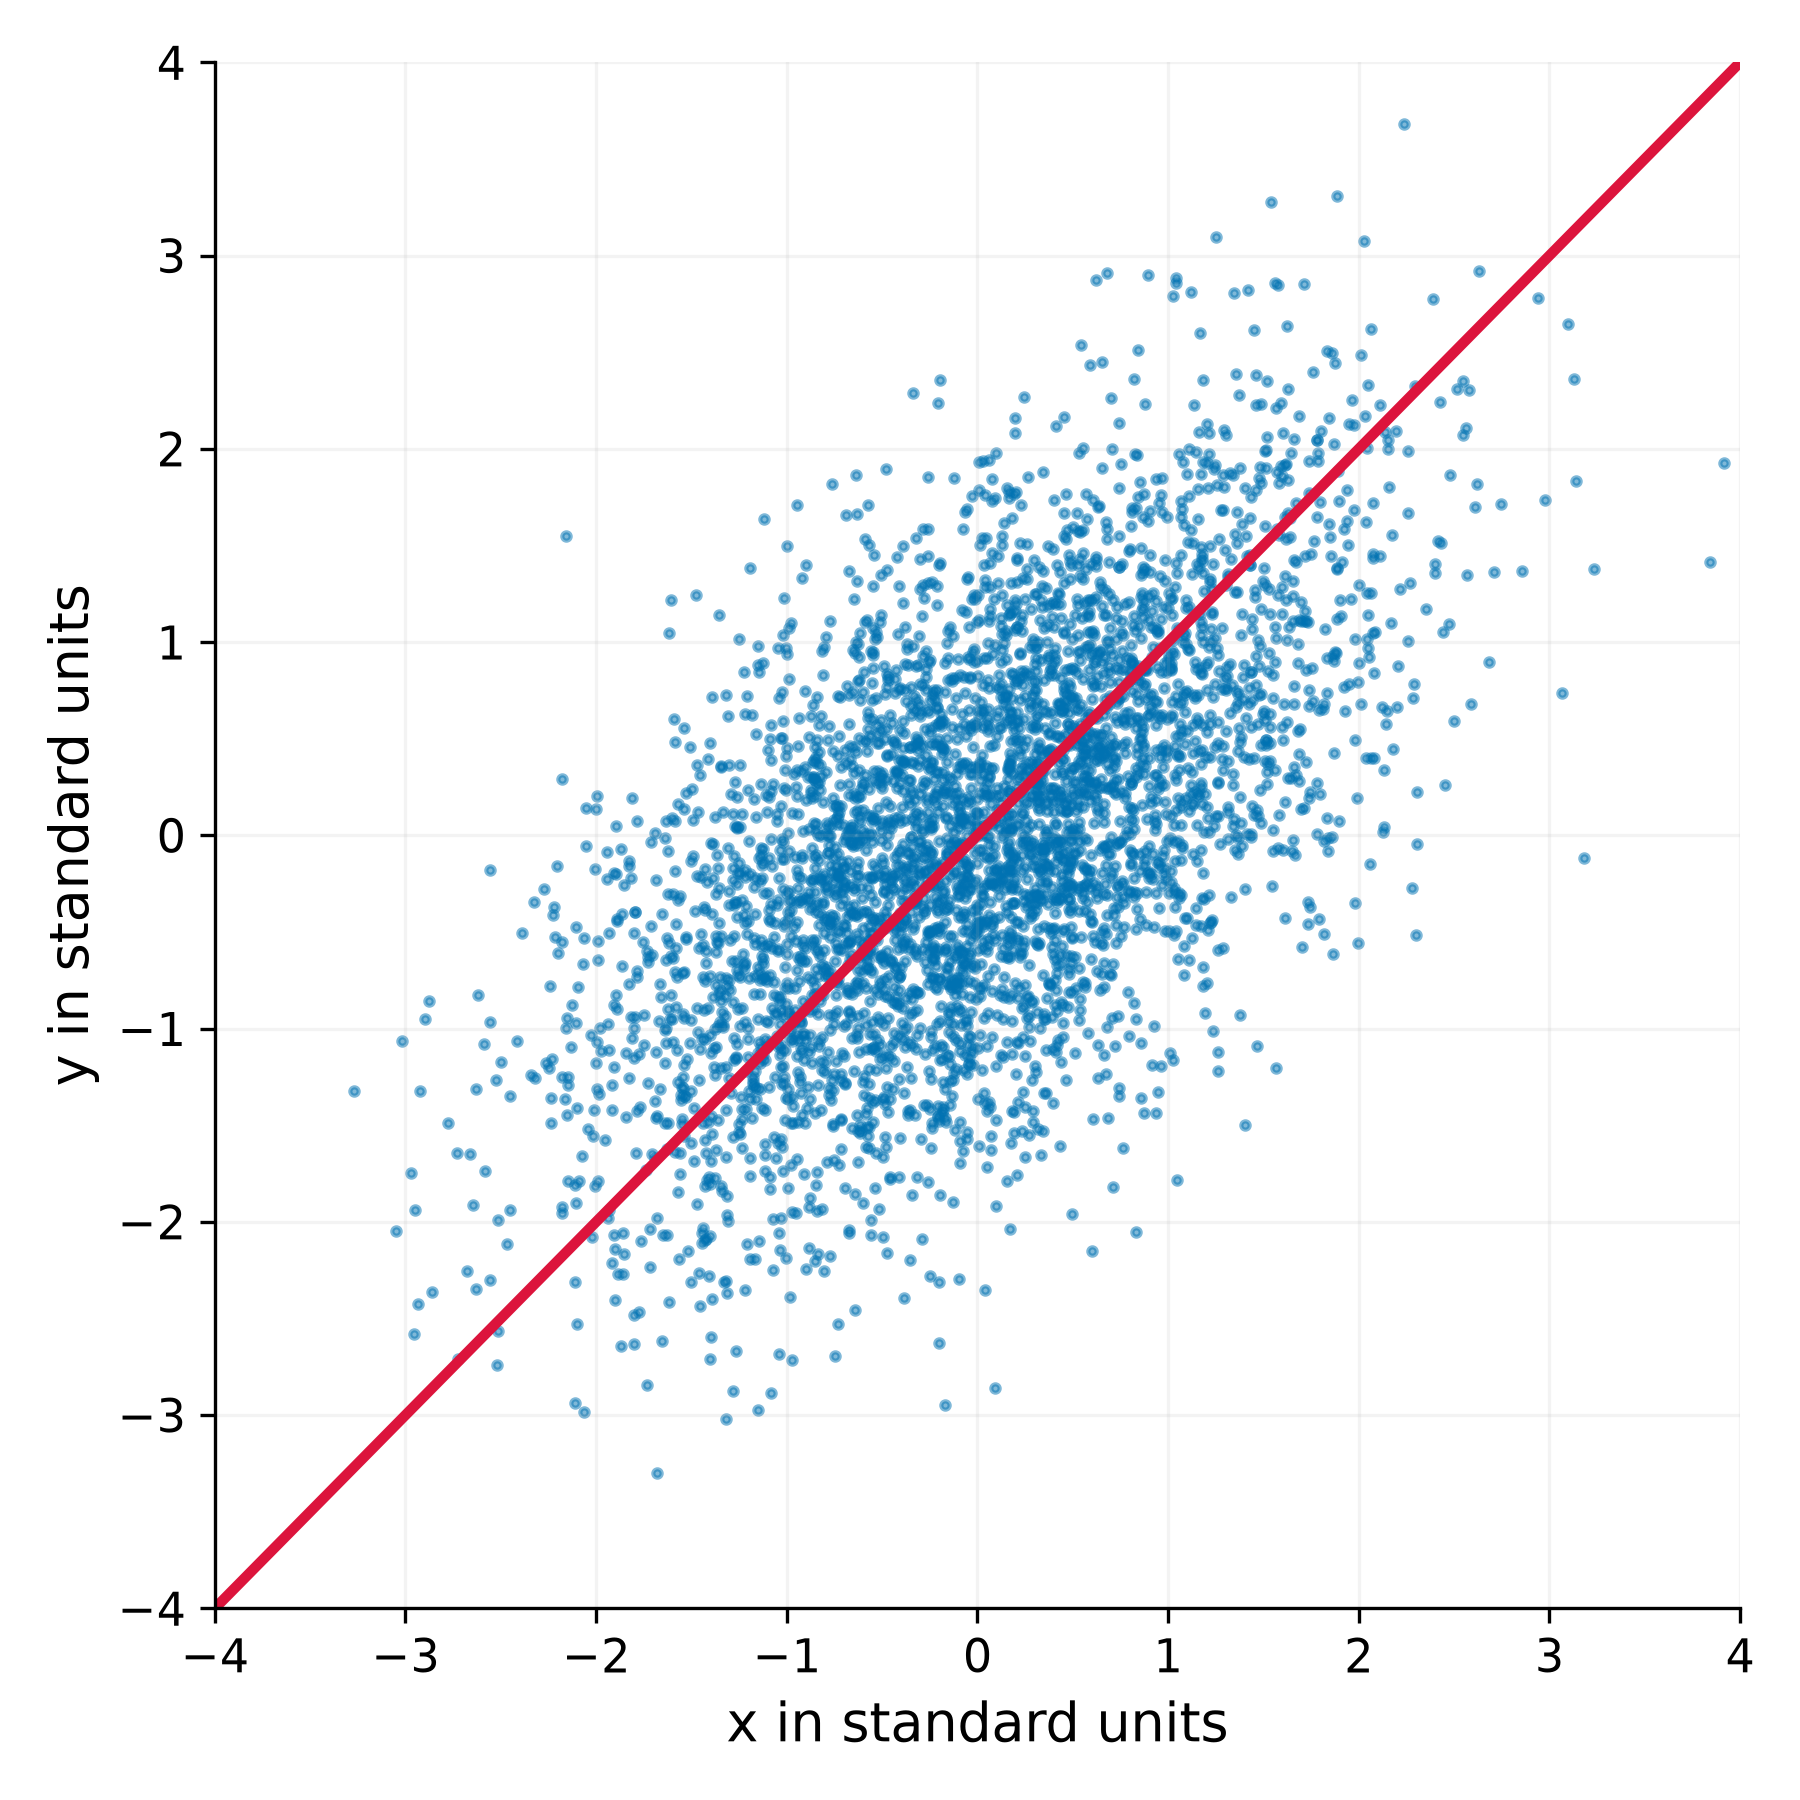
\includegraphics[width=0.95\textwidth]{grafico_linha_45.png}
        \end{column}
    \end{columns}
\end{frame}

\begin{frame}{O Efeito de Regressão (Regressão à Média)}
    \begin{itemize}
        \item Como $|r| \leq 1$, a inclinação da reta é menor ou igual a 1.
        \item \textbf{Efeito de Regressão:} A estimativa de $Y$ (em unidades padrão) estará sempre mais próxima da média do que o valor observado de $X$ (em unidades padrão).
        \item \textbf{Explicação Física:}
        \begin{itemize}
            \item Se um indivíduo apresenta uma medida extrema de $X$ (ex: $2$ desvios padrões acima da média), sua predição correspondente $\hat{Y}$ será de apenas $2 \cdot r$ desvios padrões acima da média.
            \item O fenômeno foi observado por Francis Galton em estudos de hereditariedade (pais muito altos tendem a ter filhos ligeiramente mais baixos que os pais, aproximando-se da média populacional).
        \end{itemize}
    \end{itemize}
\end{frame}

\begin{frame}{Erro de Estimativa e Função de Perda}
    \begin{itemize}
        \item Para qualquer reta de predição ajustada, existirá um \textbf{Erro de Estimativa} (ou Resíduo) para cada ponto:
        $$e_i = y_i - \hat{y}_i$$
        \item Como mensurar a qualidade de ajuste global do modelo?
        \item Definimos a \textbf{Função de Perda} (Loss Function) como a \textbf{Raiz do Erro Quadrático Médio} (RMSE):
        $$RMSE = \sqrt{\frac{1}{N} \sum_{i=1}^N (y_i - \hat{y}_i)^2}$$
        \item Onde $N$ representa o \textbf{Tamanho da Amostra}.
        \item Nosso objetivo estatístico é encontrar a reta que minimiza o valor de $RMSE$.
    \end{itemize}
\end{frame}

\begin{frame}{O Método dos Mínimos Quadrados (Least Squares)}
    \begin{itemize}
        \item O \textbf{Método dos Mínimos Quadrados} consiste em achar os parâmetros da reta que minimizam a soma dos erros quadrados de predição.
        \item Em unidades padrão, buscamos o slope $\beta_{su}$ da reta $\hat{y}_{su} = \beta_{su} \cdot x_{su}$ que minimize:
        $$L(\beta_{su}) = \frac{1}{N} \sum_{i=1}^N (y_{i,su} - \beta_{su} \cdot x_{i,su})^2$$
        \item Derivando em relação a $\beta_{su}$ e igualando a zero, prova-se analiticamente que:
        $$\beta_{su} = \frac{1}{N} \sum_{i=1}^N x_{i,su} \cdot y_{i,su} = r$$
        \item \textbf{Conclusão:} A reta de regressão em unidades padrão é a melhor reta no sentido dos mínimos quadrados.
    \end{itemize}
\end{frame}

\begin{frame}[fragile]{Exemplo Pareado: Otimização Computacional}
    \begin{block}{Minimizando o RMSE numericamente com SciPy}
\begin{lstlisting}
import numpy as np
from scipy.optimize import minimize
from scipy import stats

# Dados originais de exemplo
x = np.array([84.2, 88.1, 91.3, 85.0, 93.4])
y = np.array([89.1, 93.2, 94.5, 90.0, 97.2])

# Z-normalizacao (Unidades Padrao)
x_su = (x - np.mean(x)) / np.std(x, ddof=1)
y_su = (y - np.mean(y)) / np.std(y, ddof=1)

# Funcao de perda: RMSE
def calcular_rmse(beta, x_data, y_data):
    pred = beta[0] * x_data
    return np.sqrt(np.mean((y_data - pred) ** 2))

# Minimizacao numerica da perda
chute = [0.0]
res = minimize(calcular_rmse, chute, method='BFGS')
beta_otimizado = res.x[0]
r_analitico, _ = stats.pearsonr(x, y)

print(f"Beta Otimizado (RMSE): {beta_otimizado:.6f}")
print(f"Pearson r (Analitico): {r_analitico:.6f}")
\end{lstlisting}
    \end{block}
\end{frame}
